

\documentclass{ocbeameruni}

\setdefaultlanguage[babelshorthands=true]{german}

\newcommand{\R}{\mathbb{R}}

\title{Organic Computing 2}
\subtitle{Lösungsvorschlag Blatt09}
\date{\today}
\author{Lukas Huhn \and Qiang Chang \and Victor Gerling}
\institute{%
  Universität Augsburg\\
  Institut für Informatik\\
  Lehrstuhl für Organic Computing
}

\usepackage{listings}
\usepackage{mathtools}

\DeclarePairedDelimiter\ceil{\lceil}{\rceil}
\DeclarePairedDelimiter\floor{\lfloor}{\rfloor}

\begin{document}


\maketitle


\begin{frame}{Gliederung}
  \setbeamertemplate{section in toc}[sections numbered]
  \tableofcontents
\end{frame}


\section{Aufgabe 01}

\begin{frame}{1.1}
Passen Sie Ihre Q-Tabelle und die Interaktion mit ihr (Durchsuchen, Initialisieren, Updating
etc.) so an, dass Intervalle statt genauer Zustandswerte sowie eine Zeile pro Aktion benutzt
werden!
    \begin{itemize}
    \item States werden in Binärstrings umgewandelt, mit jeweils eigenen Min, Max und Step-values für die verschiedenen Attributte.
    \item Zum Dursuchen wurde ein Python Dictionary + Regex verwendet (langsam).
    \item Beim Update der Tabelle wurde für den Wert in Q(s, a) der Durchschnitt aller matchenden State-Action Regeln genommen. 
    \end{itemize}
\end{frame}

\begin{frame}{1.2}
Implementieren Sie einen einfachen GA für die Zustandsbeschreibungen Ihrer Q-Tabelle und
lassen Sie diesen alle paar Schritte eine Iteration durchführen! Wann läuft Ihr GA? Wie wurde
er implementiert? Welches Fitnessmaß verwenden Sie?
    \begin{itemize}
    \item Nach 50 Schritten wird der GA auf dem jetzigen Action-Set ausgeführt. 
    \item Population: 4, Selection: 2 Parents mittels Roulette-Wheel und Softmax-Distribution
    \item Uniform crossover
    \item Mutation mit 0, 1 und # (mit 0.04)
    \item Fitnessmaß: Werte der Q-Table
    \end{itemize}
\end{frame}


\begin{frame}{1.3}
Zeichnen Sie ein Episode-Returndurchschnitt-Diagramm zu FrozenLake-v0.
\begin{figure}[ht]
    \centering
    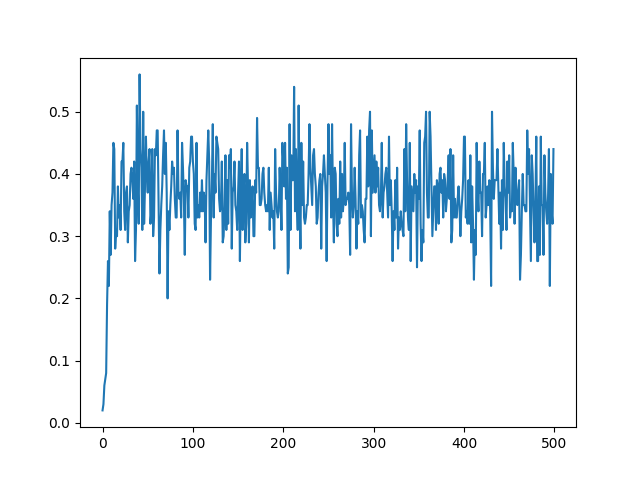
\includegraphics[width=100mm, height=60mm]{plots/frozen.png} 
\end{figure}
\end{frame}

\begin{frame}{1.4}
Zeichnen Sie ein Episode-Returndurchschnitt-Diagramm zu CartPole-v1.
\begin{figure}[ht]
    \centering
    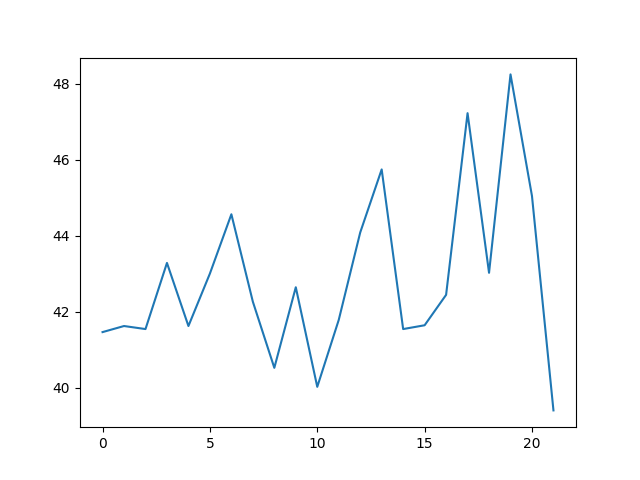
\includegraphics[width=100mm, height=60mm]{plots/cartpole_1.png} 
\end{figure}
\end{frame}

\begin{frame}{1.5}
Nach wie viel Episoden ist der Lernprozess zufriedenstellend abgeschlossen? Begründen Sie!
    \begin{itemize}
    \item Frozenlake: Bei ca. 1000, hier wird jedoch kaum generalisiert, da es ohnehin nur 16 Zustände gibt.
    \item Cartpole: Hier konnnte keine zufriedenstellende Lösung gefunden werden (evtl. falsche Parameter + ECS Lookup ist zu ineffizient)
    \end{itemize}
\end{frame}



\end{document}
% Local Variables:
% TeX-engine: xetex
% End:
